\documentclass[a4paper, 12pt]{article}%тип документа

%отступы
\usepackage[left=2cm,right=2cm,top=2cm,bottom=3cm,bindingoffset=0cm]{geometry}

%Русский язык
\usepackage[T2A]{fontenc} %кодировка
\usepackage[utf8]{inputenc} %кодировка исходного кода
\usepackage[english,russian]{babel} %локализация и переносы

%Вставка картинок
\usepackage{graphicx}
\usepackage{wrapfig}
\graphicspath{{pictures/}}
\DeclareGraphicsExtensions{.pdf,.png,.jpg}

%оглавление
\usepackage{titlesec}
\titlespacing{\chapter}{0pt}{-30pt}{12pt}
\titlespacing{\section}{\parindent}{5mm}{5mm}
\titlespacing{\subsection}{\parindent}{5mm}{5mm}
\usepackage{setspace}

%Графики
\usepackage{multirow}
\usepackage{pgfplots}
\pgfplotsset{compat=1.9}

%Математика
\usepackage{amsmath, amsfonts, amssymb, amsthm, mathtools}

%Стиль страницы
\usepackage{fancyhdr}
\pagestyle{fancy}

%ссылки
\usepackage{hyperref}

\begin{document}

\begin{titlepage}

\begin{center}
%\vspace*{1cm}
\large\textbf{Московский Физико-Технический Институт}\\
\large\textbf{(государственный университет)}
\vfill
\line(1,0){430}\\[1mm]
\huge\textbf{Работа 4.4.3}\\
\line(1,0){430}\\[1mm]
\vfill
\large Сибгатуллин Булат, ФРКТ\\
\end{center}

\end{titlepage}
\fancyhead[L] {Работа 4.4.3}
\noindent \textbf{Цель работы:}\\
\indent знакомство с работой и настройкой гониометра Г5, определение зависимости показателя преломления стекла призмы от длины волны, определение марки стекла и спектральных характеристик призмы.\\
\noindent \textbf{В работе используются:}\\
\indent гониометр, ртутная лампа, призма, стеклянная плоскопараллельная пластинка, призменный уголковый отражатель.

\section*{Экспериментальная установка}

Все измерения в данной работе производятся с помощью гониометра, он служит для точного измерения углов.

\begin{figure}[h!]
\centering
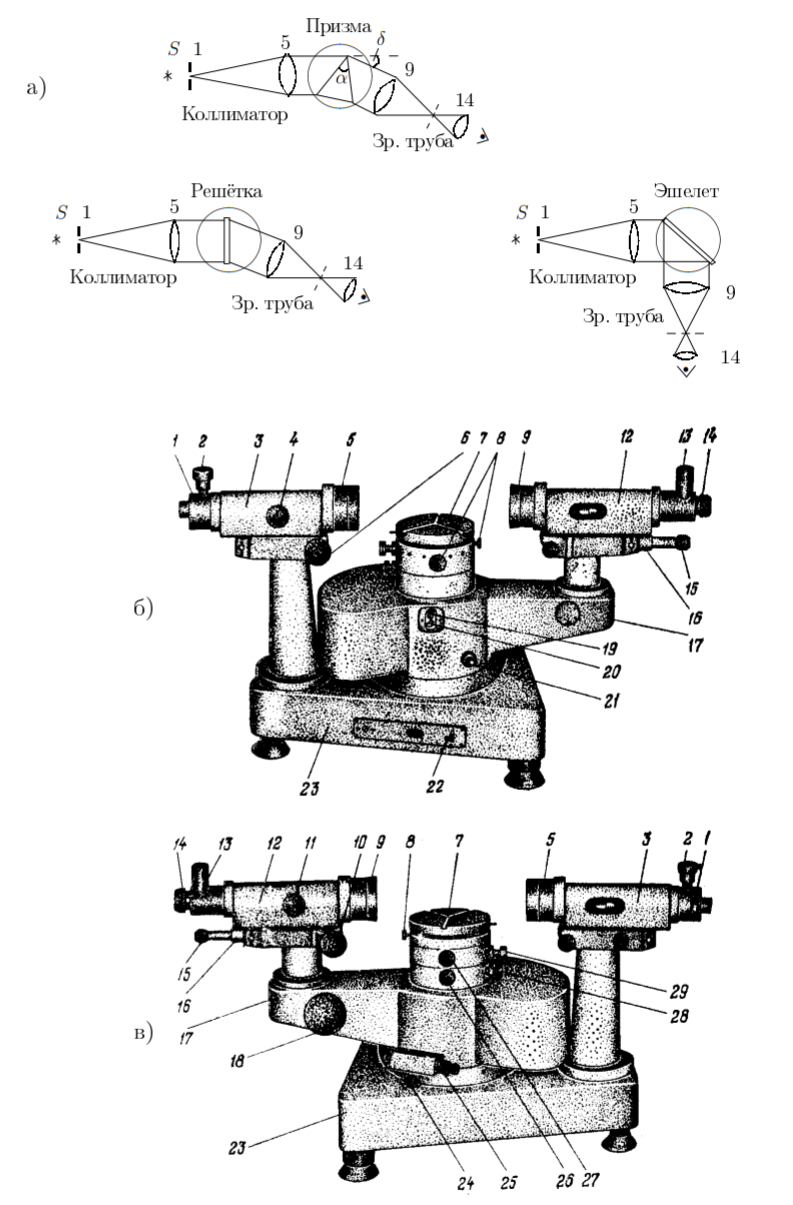
\includegraphics[scale=1]{images/scheme_1.png}
\caption{Оптическая схема и внешний вид гониометра}
\label{fig:scheme_1}
\end{figure}

Оптическая схема гониометра представлена на рис. $\ref{fig:scheme_1}$a. Свет от источника \textit{S} проходит через коллиматор и преобразуется призмой или решеткой в набор параллельных пучков, каждый из который соответсвует определленной длине волны. Параллельные пучки собираются в фокальной плоскости объектива 9 зрительной трубы и рассматриваются глазом через окуляр 14.

Внешний вид гониометра представлен на рис. $\ref{fig:scheme_1}$б и $\ref{fig:scheme_1}$в. Коллиматор 3 столик 7 и алидада 17 со зрительной трубой 12 крепятся на массивном основании 23. На столике 7 размещаются исследуемые объекты. Коллиматор закреплен неподвижно, а столик и алидада с трубой могут вращаться вокруг вертикальной оси.

Ширину коллиматорной цели можно менять при помощи микрометрического винта 2, высоту - при помощи диафрагмы с треугольным вырезом, надетой на щель. Винт 4 служит для перемещения объектива 5 - настройки коллиматора на параллельный пучок.

Зрительная труба 12 состоит из объектива 9 и окуляра 14 с автоколлимационным устройством 13. Фокусировка трубы производится винтом 11. Наклон коллиматора и зрительной трубы к горизонтальной оси изменяется винтами 6 и 10 соответственно.

\begin{wrapfigure}{r}{0.5\linewidth}
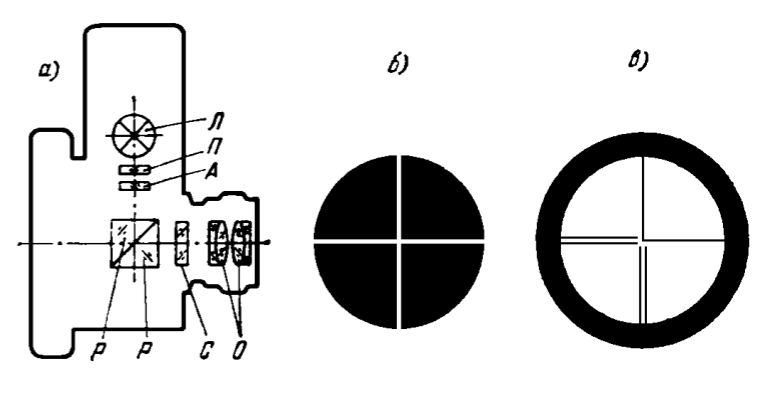
\includegraphics[scale=0.6]{images/scheme_2.png}
\caption{Автоколлимационное устройство}
\label{fig:scheme_2}
\end{wrapfigure}

Схема окуляра О зрительной трубы с автоколлимационным устройством приведена на рис. \ref{fig:scheme_2}а. Свет от лампы Л проходит через защитную стеклянную пластинку П и попадает на автоколлимационную сетку А, содержащую две взаимно перпендикулярные щели. Свет, прошедший через сетку А (светящийся крест - рис. \ref{fig:scheme_2}б), попадает на две прямоугольные призмы P и отражается от гипотенузной грани, на которую нанесён полупрозрачный слой с коэффициентом отражения 50\%.

Обе сетки окуляра, A и C (рис. \ref{fig:scheme_2}а), расположены на строго одинаковых расстояниях от гипотенузных граней призмы P, поэтому их одновременное наблюдение в окуляре возможно только при совпадении фокальных плоскостей объектива и окуляра (труба настроена на бесконечность).

Важнейшим узлом гониометра является устройство, служащее для отсчёта угла поворота зрительной трубы вокруг вертикальной оси, проходящей через центр столика. На этой оси крепится прозрачное кольцо (лимб), расположенное в корпусе прибора. На поверхности лимба нанесена шкала с делениями. Лимб разделён на $3\times 360 = 1080$ делений. Цена деления $20'$, оцифровка деления произведена через $1^{\circ}$. Шкалу лимба можно наблюдать через окуляр отсчётного устройства 16 при включённой подсветке (тумблер 22). Резкость изображения шкалы регулируется вращением оправы окуляра 15.

Оптическая система отсчётного устройства собрана так, что через окуляр можно наблюдать изображения штрихов двух диаметрально противоположных участков лимба, причём одно изображение прямое, а другое обратное (рис. \ref{fig:scheme_3}). Кроме того, оптическа система позволяется перемещать эти изображения друг относительно друга, оставляя в покое как лимб, так и алидаду со зрительной трубой. Это перемещение штрихов измеряется при помощи оптического микрометра. Шкала микрометра рассчитана таким образом, что при перемещении ееё на 600 делений верхнее изображение штрихов лимба смещается относительно нижнего на $10'$. Следовательно, цена деления шкалы микрометра $1''$.

\begin{wrapfigure}{r}{0.6\linewidth}
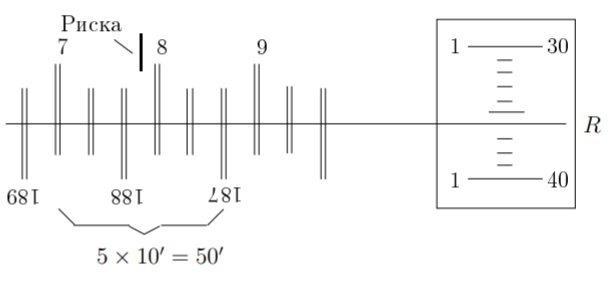
\includegraphics[scale=0.8]{images/scheme_3.png}
\caption{Поле зрения отсчётного микроскопа ($7^{\circ}51'36''$)}
\label{fig:scheme_3}
\end{wrapfigure}

Поле зрения отсчётного микроскопа приведено на рис. \ref{fig:scheme_3}. В левом окне наблюдаются изображения диаметрально противоположных участков лимба и вертикальныз штрих для отсчёта градусов, в правом - деления шкалы оптического микрометра и горизонтальная риска R для отсчёта минут и секунд.

Гониометр требует тщательной юстировки, которая заключается в установке: а) зрительной трубы на бесконечность; б) поверхности столика и оптической оси трубы - перпендикулярно оси вращения прибора; в) коллиматора - на параллельный пучок лучей; г) оптической оси коллиматора - перпендикулярно оси вращения прибора.

\section*{Теоретическая справка}

Угол отклонения материала призмы $n(\lambda )$ удобно определять по углу наименьшего отклонения $\delta (\lambda )$ (рис. \ref{fig:teor_1}). Минимальное отклонение луча, преломлённого призмой, от  направления луча, падающего на призму получается при симметричном ходе луча (в призме луч идёт параллельно основанию). Угол минимального отклонения $\delta$, преломляющий угол $\alpha$ (угол при вершине призмы) и показатель преломления связаны соотношением

\[n(\lambda) = \frac{\sin \frac{\alpha + \delta (\lambda )}{2}}{\sin \frac{\alpha}{2}}\]

\begin{figure}[h!]
\centering
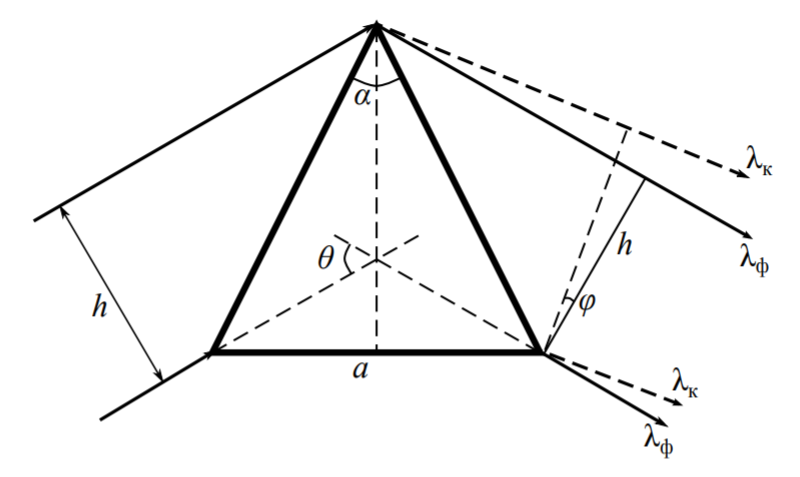
\includegraphics[scale=0.5]{images/teor_1.png}
\caption{Ход лучей в призме для наименьшего угла отклонения}
\label{fig:teor_1}
\end{figure}

\end{document}